% !TEX encoding = UTF-8 Unicode
\documentclass[10pt,ngerman]{scrartcl}
\usepackage{url,bm,tikz,a4wide}
\usepackage[utf8]{inputenc}
\usepackage{booktabs}
\usepackage{amsmath,amssymb}
\usepackage[english]{babel}
\usepackage{graphicx,tikzsymbols} 
\usepackage{xcolor}
\usepackage[numbers]{natbib}
\usepackage{float}
\usepackage{gensymb}
\usepackage{pdfpages}
\usepackage{pdflscape}
\usepackage{hyperref}

\DeclareOldFontCommand{\bf}{\normalfont\bfseries}{\mathbf}

\usepackage{nicefrac,xfrac}

\renewcommand{\theenumi}{\alph{enumi})}
\renewcommand{\theenumii}{\Roman{enumii}}

\setcounter{secnumdepth}{-1}

\begin{document}

\begin{figure}[htbp]
\begin{minipage}[b]{0.50\linewidth}
\begin{Large}
	\textbf{Group Number:} 2\newline\newline
\end{Large}
\end{minipage}
\begin{minipage}[b]{0.50\linewidth}
\begin{flushright}
\begin{Huge}
\textbf{Physics}\\
\end{Huge}
\vspace{0.5cm}
\begin{large}
Winter term 2021/22
\end{large}
\end{flushright}
\end{minipage}
\end{figure}

\vspace{2cm}
\begin{huge}
\noindent

\textbf{Group Work}
\end{huge}

\section{Momentum and Force. Fields of Force}
\subsection{A1 Neutron stars}
The so-called neutron stars have about the mass of our sun (ca. $2 \cdot 10^{30}kg$) and a typical diameter of about 20 km. Their mean mass density is roughly that of an atomic nucleus.

\begin{enumerate}
	\item How big is the mean mass density?
	\begin{align*}
		V_{Sphere} &= (\frac{4}{3}) \cdot \pi \cdot r^3\\
		p &= \frac{m}{V} = \frac{m}{(\frac{4}{3}) \cdot \pi \cdot r^3}\\
		p &= \frac{2 \cdot 10^{30}kg}{(\frac{4}{3}) \cdot \pi \cdot (10000m)^3} = 4.775 \cdot 10^{17} kg/m^3 \\
	\end{align*}
	The mean mass of a neutron star is approximately $4.775 \cdot 10^{17} kg/m^3$ \newline
	
	\item According to Newton's law of gravitation, how heavy would a piece of weight with the mass of 1kg be on the surface of a neutron star?
	\begin{align*}
		W &= m * g \\
		g &= G * \frac{M}{R^{2}} \\
		g &= 6,67 * 10^{-11} N * \frac{kg^{2}}{m^{2}} * \frac{2*10^{30} kg}{10^{8} m^{2}} = 1,334 * 10^{18} \frac{m}{s^{2}} \\
		W &= 1kg * 1,334 * 10^{18} \frac{m}{s^{2}} = 1,334 * 10^{18} N \\
	\end{align*}
	\newpage
	\item How heavy would $1mm^3$ of neutron star matter be on earth and what diameter would an iron ball of the same mass have?
	\begin{align*}
		m &= V * p \\
		W &= m * g \\
		m &= 10^{-9} m^{3} * 4,77 * 10^{17} \frac{kg}{m^{3}} = 4,77 * 10^{8} kg \\
		W &= 4,77 * 10^{8} kg * 9,81 \frac{m}{s^{2}} = 4,68 * 10^{9} N \\
		V &= \frac{m}{p} \\
		r &= \sqrt[3]{\frac{V * 3}{4\pi}} \\
		p &= 7,6 * 10^{3} \frac{kg}{m^{3}} \\
		V &= \frac{4,68 * 10^{9} N}{7,6 * 10^{3} \frac{kg}{m^{3}}} = 6,15 * 10^{5} m^{3} \\
		r &= \sqrt[3]{\frac{6,15 * 10^{5} m^{3} * 3}{4\pi}} = 52,75 m \\
		d &= 2 * r = 105,5 m \\
	\end{align*}
\end{enumerate}

\subsection{A2 Coulomb interaction of two electrons}
Sketch correctly to scale the course of the magnitude of the force with which two electrons repel each other at distances of $0,5 \cdot 10^{-10}$m to $5,0 \cdot 10^{-10}$m according to Coulomb's law.
\begin{align*}
	[Q] &= As \\
	Q &= n * e \\
	e &= 1.6022 * 10^{-19} As \\
	Q_{1} &= Q_{2} = e = 1.6022 * 10^{-19} As \\
	\epsilon &= \epsilon_{0} * \epsilon_{r} \\
	\epsilon_{0} &= 8.854 * 10^{-12} \frac{As}{Vm} \\
	\epsilon_{r} &= 1 \text{ (vaccuum)}\\
	\vec{F_{Q1}} &= \frac{1}{4 * \pi * \epsilon } * \frac{Q_{1}*Q_{2}}{r^{2}} * \frac{\vec{r}_{12}}{|\vec{r}_{12}|} = -\vec{F_{Q2}} \\
	F_{Q1} &= \frac{1}{4 * \pi * \epsilon } * \frac{Q_{1}*Q_{2}}{r^{2}} = -F_{Q2}
\end{align*}
See sketch on next page and calculation of data points in appendix \hyperref[sec:data-table-a2]{3.1 Data table 1.2 (A2)}

\begin{landscape}
 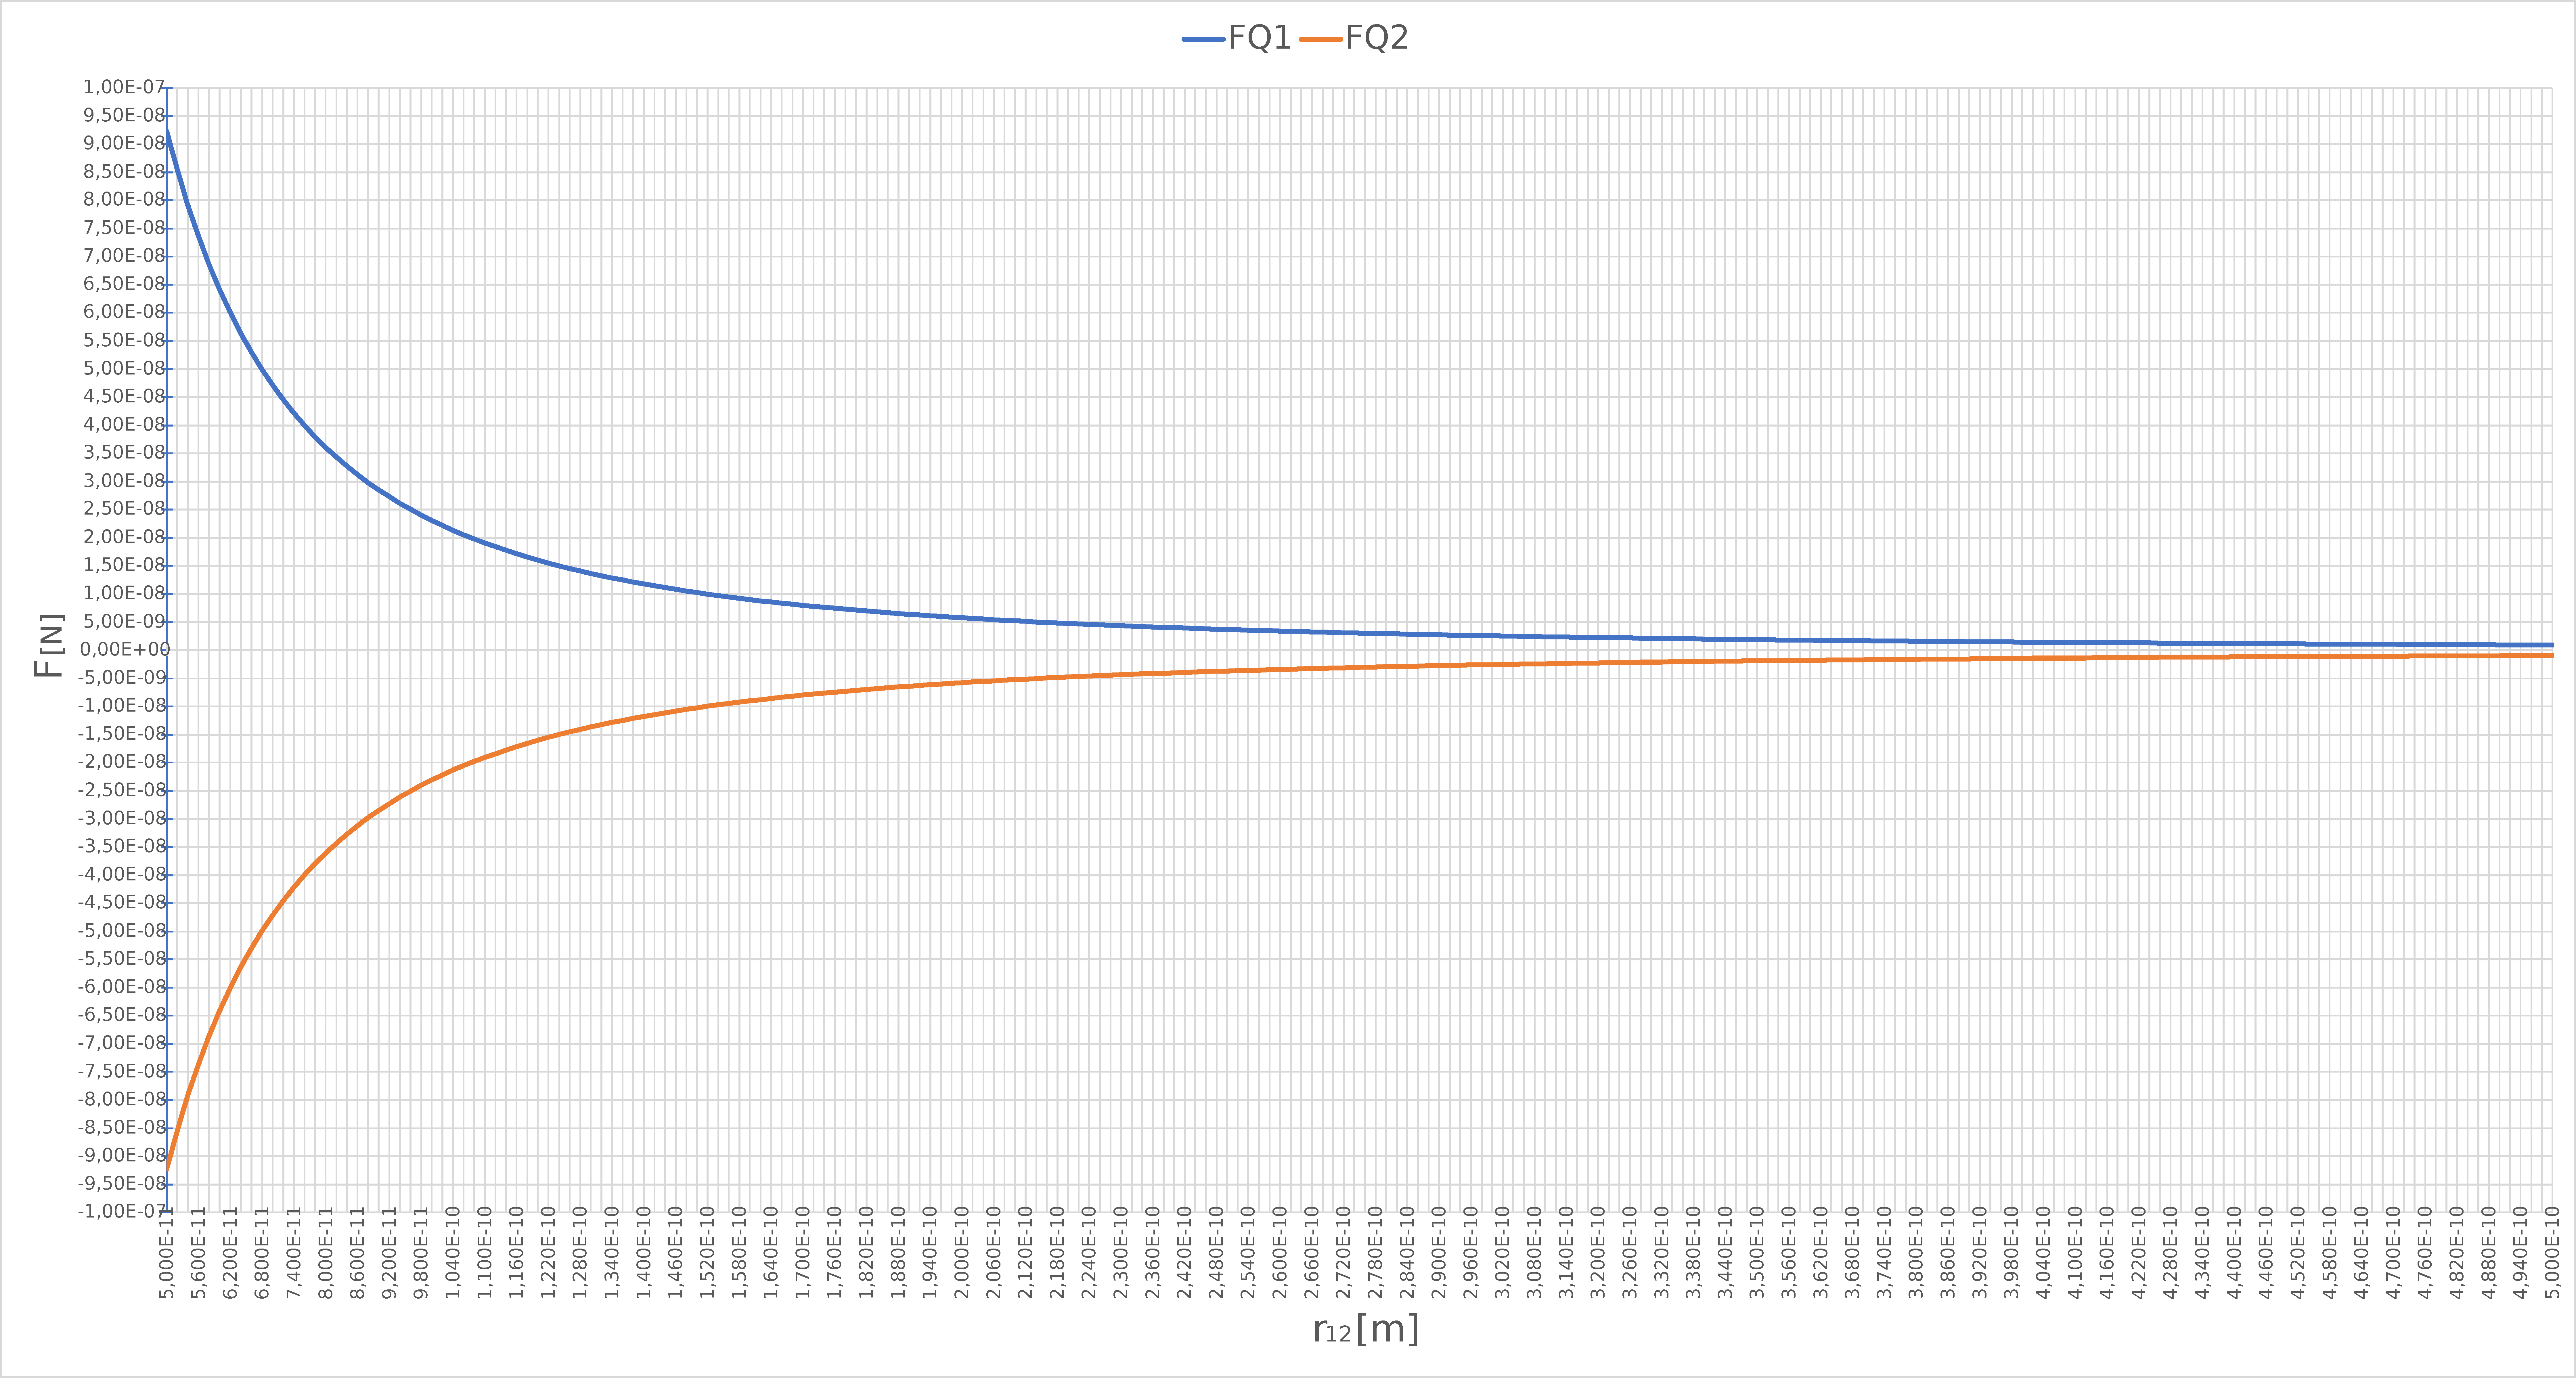
\includepdf[pages={-},angle=90]{force_a2.pdf}
\end{landscape}

\newpage
\section{Work and Power. Energy. Heat and Temperature}
\subsection{B1 train set}
For example, the electric drive of a train set consumes the power shown in the figure below during a operational cycle (1 MW = 106 W).

\begin{enumerate}
	\item What is the total electrical energy consumed during this operational cycle?
	\begin{align*}
		P_{1} &= \frac{7MW\cdot 120s}{2} = 420MWs = 420MJ\\
		P_{2} &= 2 MW * 600s = 1200 MW = 1.2 GJ\\
		P_{3} &= \frac{-7MW * 60s}{2} = -240 MW\\
		P_{total} &= P_{1} + P_{2} + P_{3} = 420MJ + 1.2 GJ - 240 MJ = 1.38 GJ
	\end{align*}
	\item What is the mean power consumed?
	\begin{align*}
        P_{mean} = \frac{P_{total}}{\Delta t} = \frac{1.38 GJ}{\Delta t_{1} +\Delta t_{2} +\Delta t_{3} +\Delta t_{4}}
		= \frac{1.38GWs}{120s + 600s + 60s + 60s} = 1.643MW
  \end{align*}
\end{enumerate}

\begin{figure}[H]
	\centering
	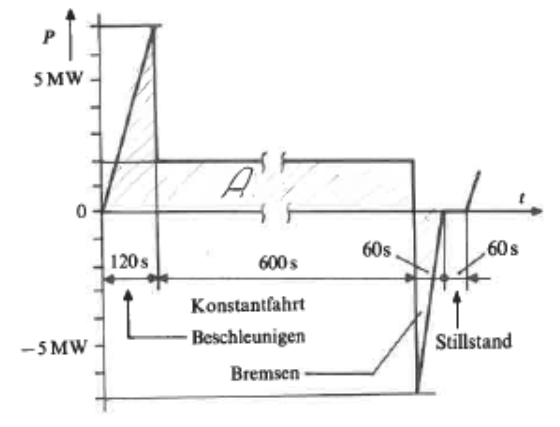
\includegraphics[scale=0.5]{group_work_1.png}
\end{figure}

\section{B2 crash test facility}
In a crash test facility, a vehicle including cuts m = 900 kg is accelerated uniformly via an electric linear motor through a distance s = 20 m with a constant force F = 5 kN.
\begin{enumerate}
	\item[1] How big is the necessary electrical energy in kWh if all losses are neglected?
	\item[2] How big is the final speed achieved?
	\item[3] During the subsequent impact process, the vehicle is brought to a standstill within a distance of s = 80 cm. What is the mean force that acts on a fictitious seated occupant, m1 = 80 kg?
\end{enumerate}
1. 
	\begin{align*}
			m &= 900 kg \\
			s &= 20 m \\
			F &= 5000N \\
			F &= m * a \rightarrow a = \frac{F}{m} \\
			a &= \frac{F}{m} = \frac{5000N}{900kg} = 5.556 \frac{m}{s^{2}} \\
			s &= 0.5 * a * t^{2} \rightarrow t = \sqrt{\frac{s}{0.5 * a}} \\
			t &= \sqrt{\frac{s}{0.5*a}} = \sqrt{\frac{20m}{0.5 * 5.556 \frac{m}{s^{2}}}} = 2.68s \\
			P &= \frac{F * s}{t} = \frac{5000m * 20 m}{2.68s} = 37 313.4328358209 W \\
			Energy &= P * t = 37 313.4328358209 W * 2.68s = 100000Ws = 0.0278kWh \\
			\intertext{or}
			W &= F * d = 5000N * 20m = 100000 = \frac{100000}{3.6 * 10^6} = 0,028 kWh
	\end{align*}
2.
	\begin{align*}
		v &= a * t = 5.556 \frac{m}{s^{2}} * 2.68s = 14.889 \frac{m}{s} \widehat{=} 53,6 kmh \\		
	\end{align*}
3.
	\begin{align*}
		m &= 900 kg \\
		s &= 0.8 m \\
		v &= 14.889 \frac{m}{s} \\
		a &= - \frac{v^{2}}{2*s} = - \frac{(14.889 \frac{m}{s})^{2}}{2*0.8m} = -138.55 \frac{m}{s^{2}} \\
		F &= m * a = 80 kg * 138.55 \frac{m}{s^{2}} = 11084 N
	\end{align*}
\section{B3 Connected load of a flow heater}
Suppose you want to design an electric water heater without a storage tank that heats a water flow of 0,1 l/s from 10 °C to 60 °C. 
What is the minimum required electrical connection power? (specific heat capacity of water c = 4,19 kJ/(kgK)).
\newline
\begin{align*}
	T_{in} &= 10\degree C \\
	T_{out} &= 60\degree C \\
	\Delta T &= 50^{\degree}C = 50K \\
	\text{water flow} &= 0.1\frac{l}{s} \\
	m &= 0.1kg \\
	\intertext{specific heat capacity of water c} 
	c &= 4.19kJ/(kgK) \\
	\intertext{total energy to heat up 0.1l water}
	\Delta Q &= c \cdot m \cdot \Delta T \\
	\intertext{minimum required electrical connection power} 
	[W] &= kWh \\
	\intertext{Required energy to heat up 0.1 kg water from $10\degree$C to $60\degree$C}
	\left[\Delta Q\right] &= K \cdot kg \cdot \frac{kJ}{kg \cdot K} = kJ \\
	\Delta Q &= 50 \cdot 0.1 \cdot 4.19 = 20.95kJ \\
	\intertext{Required connection power to heat up 0.1l/s water from $10\degree$C to $60\degree$C}
	\left[P\right] &= W \\
	P &= \frac{E}{t_{s}} \\
	\intertext{($t_{s}\rightarrow$ time period in seconds $\rightarrow$ in this case one second because of heating up the specific amount of water every second)}
	P &= \frac{20950}{1} = 20950W = 20.95kW
\end{align*}

\newpage
\section{Appendix}
\subsection{Data table A2}
\label{sec:data-table-a2}
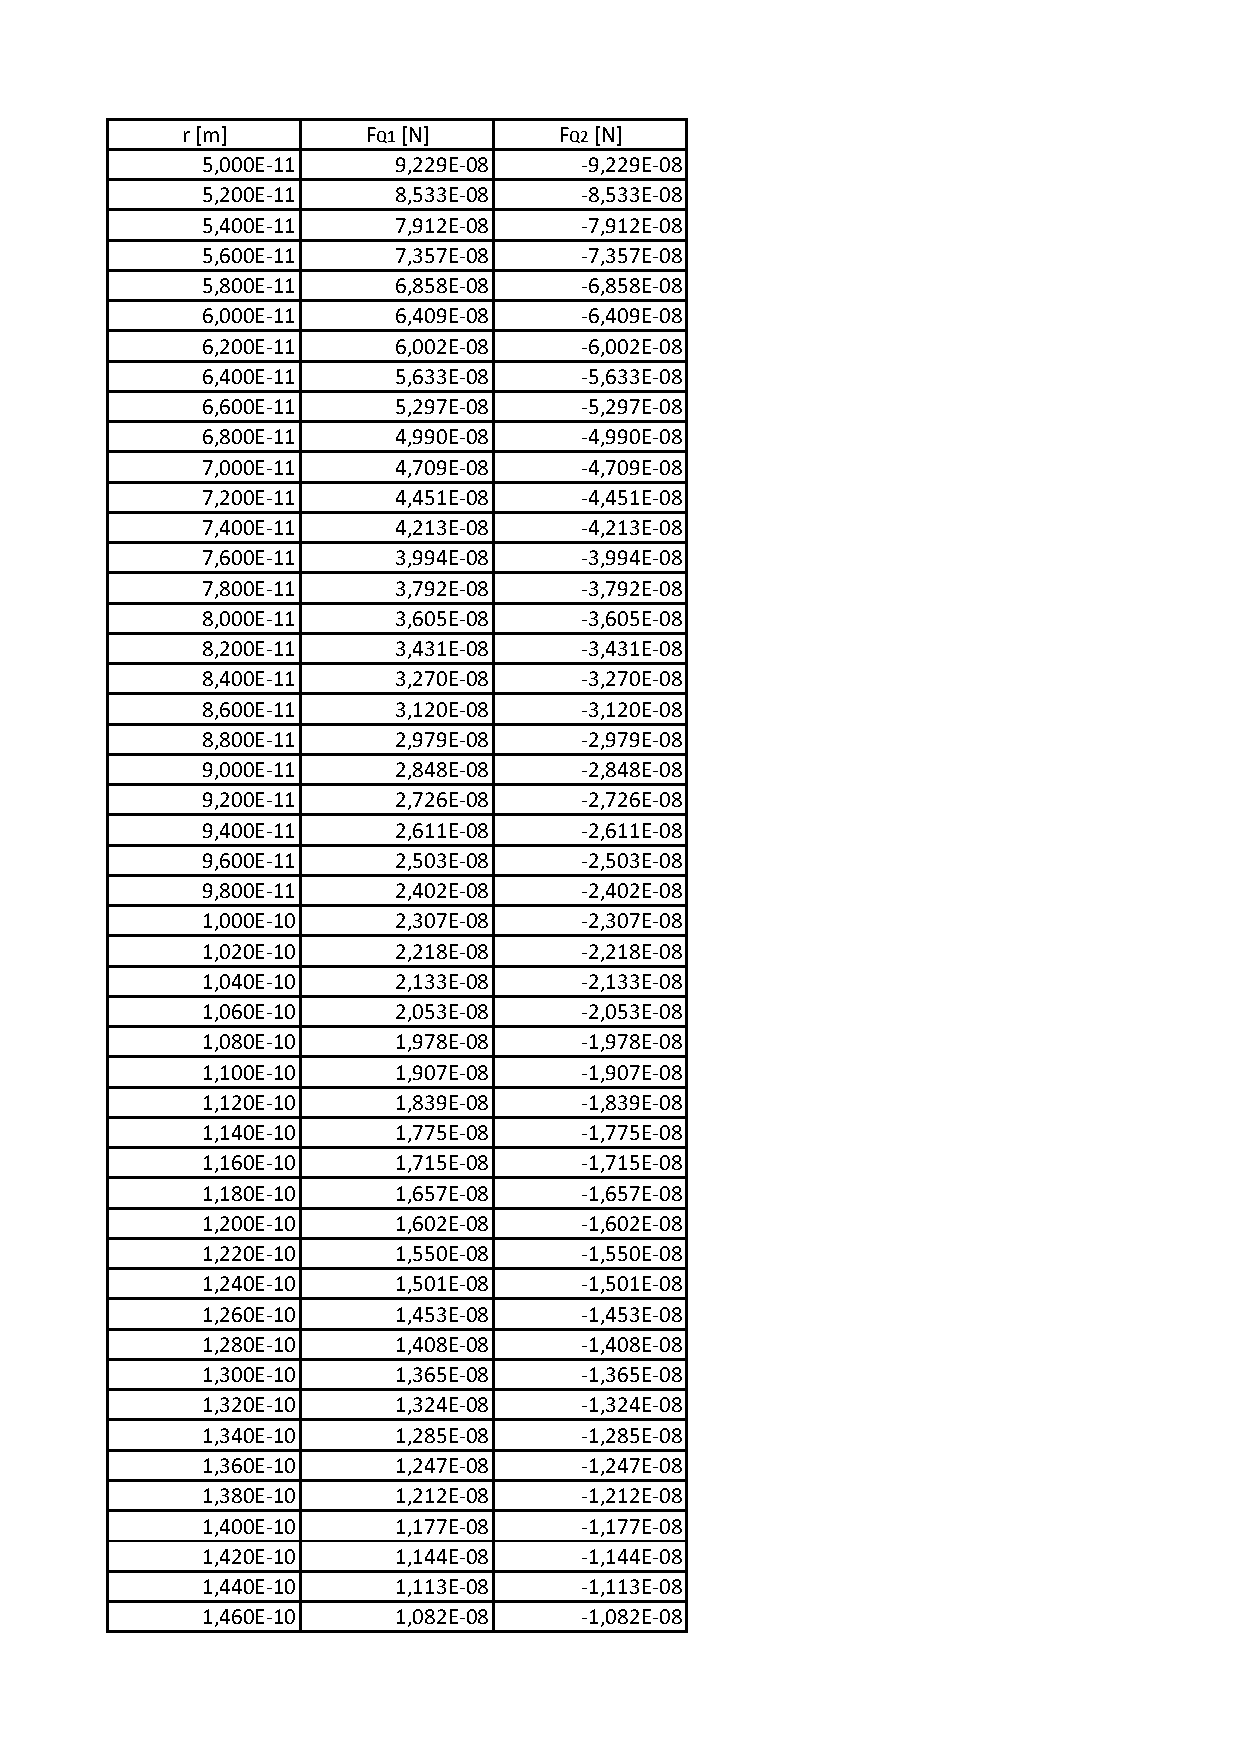
\includepdf[pages=-]{a2_table.pdf}

\end{document}